%------------------------------------------------------------------------------
% Template file for the submission of papers to IUCr journals in LaTeX2e
% using the iucr document class
% Copyright 1999-2003 International Union of Crystallography
% Version 1.2 (11 December 2002)
%------------------------------------------------------------------------------

\documentclass[preprint]{iucr}              % DO NOT DELETE THIS LINE
%\documentclass{article}
\usepackage{lscape}
\usepackage[centertags]{amsmath}
\usepackage{amsfonts}
\usepackage{amssymb}
\usepackage{amsthm}
\newcommand{\mb}[1]{\ensuremath{\mbox{\boldmath $ #1 $}}}
\newcommand{\mbss}[1]{\ensuremath{\mbox{\boldmath $ \scriptstyle #1 $}}}
\newcommand{\av}[1]{\ensuremath{\langle #1 \rangle}}
\newcommand{\dubint}{\int\!\!\!\int}
\newcommand{\intZ}{\int\!\!\!\int}
     %-------------------------------------------------------------------------
     % Information about the type of paper
     %-------------------------------------------------------------------------
     \paperprodcode{a000000}      % Replace with production code if known
     \paperref{xx9999}            % Replace xx9999 with reference code if known
     \papertype{FA}               % Indicate type of article
                                  %   FA - research papers (full article)
                                  %   SC - short communications
                                  %   FC - fast communications
                                  %   LA - lead article
                                  %   TR - topical review
                                  %   XL - crystallization papers
                                  % (Following categories rarely in LaTeX)
                                  %   AA - abstracts
                                  %   AD - addenda and errata
                                  %   AI - inorganic compounds
                                  %   AM - metal-organic compounds
                                  %   AO - organic compounds
                                  %   BC - books received
                                  %   BR - book reviews
                                  %   BI - biography
                                  %   CA - cif applications
                                  %   CD - crystal data
                                  %   CE - current events
                                  %   CI - inorganic compounds
                                  %   CL - calendar of events
                                  %   CM - metal-organic compounds
                                  %   CN - cryocrystallography papers
                                  %   CO - organic compounds
                                  %   CP - computer programs
                                  %   CR - crystallographers
                                  %   CS - scientific comment
                                  %   ED - editorial
                                  %   EI - inorganic compounds
                                  %   EM - metal-organic compounds
                                  %   EO - organic compounds
                                  %   FI - inorganic compounds
                                  %   FM - metal-organic compounds
                                  %   FO - organic compounds
                                  %   IP - issue preface
                                  %   IU - iucr
                                  %   LE - letters to the editor
                                  %   LN - laboratory notes
                                  %   ME - forthcoming meetings/short courses
                                  %   MR - meeting reports
                                  %   NN - notes and news
                                  %   NP - new commercial products
                                  %   OB - obituaries
                                  %   PA - computer program abstracts
                                  %   RI - reference information
                                  %   SG - structural genomics papers
                                  %   SI - short format inorganic compounds
                                  %   SM - short format metal-organic compounds
                                  %   SO - short format organic compounds
                                  %   SP - short structural papers
                                  %   SR - software reviews
                                  %   TE - teaching and education

     \paperlang{english}          % Can be english, french, german or russian
     %-------------------------------------------------------------------------
     % Information about journal to which submitted
     %-------------------------------------------------------------------------
     \journalcode{A}              % Indicate the journal to which submitted
                                  %   A - Acta Crystallographica Section A
                                  %   B - Acta Crystallographica Section B
                                  %   C - Acta Crystallographica Section C
                                  %   D - Acta Crystallographica Section D
                                  %   E - Acta Crystallographica Section E
                                  %   J - Journal of Applied Crystallography
                                  %   S - Journal of Synchrotron Radiation
          %--------------------------------------------------------------------
          % The following entries will be changed as required by editorial staff
          %--------------------------------------------------------------------
     \journalyr{2003}
     \journaliss{1}
     \journalvol{59}
     \journalfirstpage{000}
     \journallastpage{000}
     \journalreceived{0 XXXXXXX 0000}
     \journalaccepted{0 XXXXXXX 0000}
     \journalonline{0 XXXXXXX 0000}

\begin{document}                  % DO NOT DELETE THIS LINE

     %-------------------------------------------------------------------------
     % The introductory (header) part of the paper
     %-------------------------------------------------------------------------

     % The title of the paper. Use \shorttitle to indicate an abbreviated title
     % for use in running heads (you will need to uncomment it).

\title{Molecular Crystal Global Phase Diagrams III: Sufficient parameter space determination}
%\shorttitle{Short Title}

     % Authors' names and addresses. Use \cauthor for the main (contact) author.
     % Use \author for all other authors. Use \aff for authors' affiliations.
     % Use lower-case letters in square brackets to link authors to their
     % affiliations; if there is only one affiliation address, remove the [a].

\cauthor[a,b]{J. Brandon}{Keith}
\author[a]{Richard B.}{McClurg}{mcclurg@cems.umn.edu}

\aff[a]{Department of Chemical Engineering and Materials Science,
University of Minnesota, Minneapolis, Minnesota} \aff[b]{Department
of Physics and Astronomy, Brigham Young University, Provo, Utah}

     % Use \shortauthor to indicate an abbreviated author list for use in
     % running heads (you will need to uncomment it).

%\shortauthor{Soape, Author and Doe}

     % Use \vita if required to give biographical details (for authors of
     % invited review papers only). Uncomment it.

%\vita{Author's biography}

     % Keywords (required for Journal of Synchrotron Radiation only)
     % Use the \keyword macro for each word or phrase, e.g.
     % \keyword{X-ray diffraction}\keyword{muscle}

%\keyword{keyword}

     % PDB and NDB reference codes for structures referenced in the article and
     % deposited with the Protein Data Bank and Nucleic Acids Database (Acta
     % Crystallographica Section D). Repeat for each separate structure e.g
     % \PDBref[dethiobiotin synthetase]{1byi} \NDBref[d(G$_4$CGC$_4$)]{ad0002}

%\PDBref[optional name]{refcode}
%\NDBref[optional name]{refcode}

\maketitle                        % DO NOT DELETE THIS LINE

\begin{synopsis}
A representative potential is reverse engineered for all ordered
single component tetrahedral molecule crystals in the CSD.
\end{synopsis}

\begin{abstract}
In previous papers~\cite{Mettes04,McClurg05} we developed a method
for constructing global phase diagrams (GPDs) for molecular crystals
and partially applied it to identifying reference lattices
pertaining to all single component ordered crystal structures of
tetrahedral molecules in the Cambridge Structural Database. Here we
expand upon these results by outlining a method to derive a
representative potential characteristic of all experimental
structures in our data set. This is significant because our prior
work~\cite{Mettes04} did not specify the number of parameters needed
for GPDs. Although there are suggestions in the literature that
thousands of parameters are required to adequately describe
tetrahedral molecule intermolecular potentials~\cite{Briels80}, we
find 15 parameters are sufficient to successfully plot the
structures of our test data on molecular crystal GPDs.
\end{abstract}

\pagebreak

     %-------------------------------------------------------------------------
     % The main body of the paper
     %-------------------------------------------------------------------------
     % Now enter the text of the document in multiple \section's, \subsection's
     % and \subsubsection's as required.

\section{Introduction}

Supramolecular organic solids and mesophases are of primary interest
in pharmaceuticals, electrophotographic processes, organic pigments
and dyes, and molecular FET's and dielectrics~\cite{Bassoul00}. To
alter their electrical, optical, thermal, and solubility properties
it is necessary to design both the molecular and supramolecular
structure to produce novel, application-specific materials. While
standard quantum chemistry methods are adequate for predicting
molecular properties, the weak interactions responsible for
determining supramolecular structure are more difficult to
design~\cite{Lommerse00,Motherwell02}.

Previous work~\cite{Keith04c,Mettes04} has demonstrated the ability
to construct global phase diagrams (GPDs) which can be used for
materials design by displaying the types of structures obtained from
all possible supramolecular potentials. GPDs use an
intermolecular potential constructed from a complete set of basis
functions for rotational space for all molecules of a particular
point group and a set of molecular center-of-mass packings derived
in a companion paper~\cite{McClurg05}. The parameters of the
intermolecular potential become axes on GPDs for each packing and
the crystal structures are phase regions in the diagrams.

An important benchmark of GPD's utility is to show that
experimentally observed structures can be found and their
intermolecular potential parameters read from the axes.
In a companion paper~\cite{McClurg05} we found our data set consisting of
all ordered single-component crystal structures of
tetrahedral molecules in the Cambridge Structural Database
(CSD)~\cite{Allen02} have molecular centers of mass situated on
high symmetry space groups, or reference lattices. Our goal
in this paper is to determine the number of potential parameters needed
to find all experimental phases of this data set on GPDs pertaining to these
reference lattices.  A small number of each will
disprove previous hypotheses that many parameters are
needed to describe intermolecular potentials~\cite{Briels80}
and will enhance the useability of GPDs in
materials design. The remainder of this paper is as follows. In Sec.~\ref{method} we
review the rotational potential and outline the computational
procedure to find potential parameters for each structure. This
is done using global optimization techniques among parameter
\emph{and} configurational space. In Sec.~\ref{discussion} we
discuss the reverse-engineered potentials and some aspects of our model. We end with a conclusion
about our results.

%In this paper we determine potential parameters for
%single-component tetrahedral molecules in the Cambridge Structural
%Database (CSD)~\cite{Allen02}.  We first identify the
%high-symmetry lattice formed by the molecular centers of each
%experimental structure. This gives us a starting point or
%reference lattice from which GPD's were constructed previously.
%The rotational potential is then expanded in a complete set of
%basis functions whose potential coefficients are independent
%variables on GPD's.  In this paper however we map these to the
%n-sphere and search among them for the correct or observed crystal
%structure.  This is done using global optimization techniques
%among parameter \emph{and} configurational space.

\section{Representative Potential Determination}
\label{method}

Global phase diagrams require (1) reference lattices consistent with
molecular centers of mass in experimental structures and (2)
intermolecular potential (IP) parameters to use as independent
parameters. In \cite{McClurg05} we found the majority of the
experimental structures in the CSD of tetrahedral molecules can be
classified using only five reference lattices. Since there is little
data for other reference lattices, we focus on the set \{bcc, fcc,
hcp, A5$^\prime$, sc\}. Each of these has at least four monomer
crystal structures in the data set. In this section we seek to
determine a \emph{sufficient} parameter space such that experimental
structures are each stable in a separate subspace. Thus we review
our choice of IP and define the potential parameters.  Then we
outline a method for identifying representative potential parameters
for each experimental structure. This is done using a low
temperature structural limit which is convenient and consistent with
with the experimental database but is not strictly necessary.  Then
the IP is truncated to create a finite dimensional IP parameter
space.  A library of alternative crystal structures is constructed
with which to compare experimental structures, and a figure of merit
is specified when searching for the potential parameters. This
procedure identifies a structure with similar cell shape, molecular
center of mass, and molecular orientations as shown in
Fig.~\ref{compare}.

%Having assigned reference lattices for the experimental data set
%in Sec.~\ref{assignments}, we describe a method of reverse
%engineering a representative potential responsible for the observed
%orientational ordering of the molecules on their reference
%lattice. Such a potential would be characteristic of a family of potentials
%consistent with an experimental structure and would be located in a subset of parameter space
%lower in energy than potentials of all other structures.  We expect the size in potential parameter
%space of each family to be rather small due to extreme parameter sensitivity
%is discussed in Refs.~\cite{Keith04c,Mettes04}.

%A comparison of an experimental
%structure with a structure using the potential parameterization we have chosen is shown in Fig.~\ref{compare}. Similar unit cell
%shape and molecular orientation indicates the reference lattice is
%close to the experimental lattice and the rotational ordering is
%similar to the observed molecular orientations. To outline the procedure for obtaining such a potential we
%review the mathematical model and potential
%parameters, discuss a figure of merit for searching parameter
%space, and then describe a computational strategy to optimize the
%parameters.

\begin{figure}
\scalebox{.38}{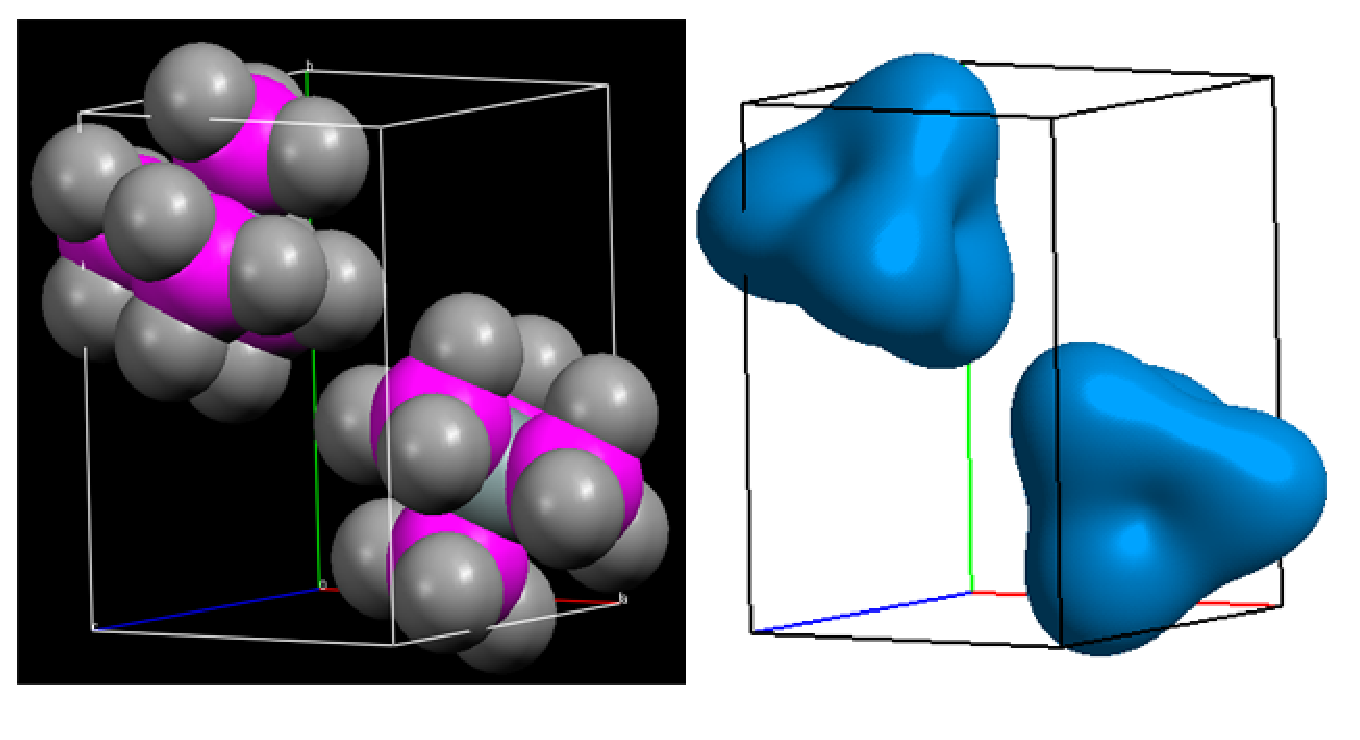
\includegraphics{mezdieCompareII.eps}}
\caption{Comparison of an experimental structure,
tetrakis(trimethystannyl)silane  [CSD structure MEZDIE01], which
crystallizes in space group 2 at Wyckoff point i with
arbitrarily-shaped tetrahedral figures whose orientation is
determined by orientational energy minimization with molecular
center of mass on an ideal bcc reference lattice.\label{compare}}
\end{figure}

\subsection{Mesoscopic Hamiltonian}
\label{hamiltonian}

Previously~\cite{Mettes04} we discussed the construction of a
nearest neighbor rotational potential for van der Waals molecules.
It is a level of abstraction above an atom-atom or site-site
potential but retains a firm basis in quantum
mechanics~\cite{Avoird94}. The potential consists of a two center
expansion constructed by coupling one center basis functions
$U^{\ell_i}_{m_\tau n_\sigma}$ for pairs of molecules $i$ and $j$
and coupling ``matrix" $J_{m_\tau n_\sigma m_\rho n_\mu}^{\ell_i
\ell_j}$,
\begin{eqnarray}
\label{re:eq:vij2}V_{\mathrm{or}} &=&
\frac{1}{2}\sum_{ij}\sum_{\ell_i\ell_j m_\tau m_\rho n_\sigma n_\mu}
U^{\ell_i}_{m_\tau n_\sigma}(\mb{\omega}_i)\nonumber\\
&&{}\times J_{m_\tau n_\sigma m_\rho n_\mu}^{\ell_i
\ell_j}(\mb{\nu},\mb{\Omega}_{ij})U^{\ell_j}_{m_\rho
n_\mu}(\mb{\omega}_i).
\end{eqnarray}
The one half avoids overcounting, $\ell_i,\ell_j\in\mathbb{N}$, the
natural numbers, and $|\ell_i-\ell_j|\leq\ell\leq \ell_i+\ell_j$.

$U^{\ell_i}_{m_\tau n_\sigma}(\mb{\omega}_i)$ are functions of the
orientation of the molecule through its Euler angles $\mb{\omega}_i$
using the passive convention~\cite{Varshalovich88}.  They are
projected from SO(3) irreducible representations (IR's), also called
Wigner functions, and contain both the point group symmetry of the
molecule and that of the Wyckoff point in the crystal,
\begin{equation}
\label{re:eq:rotfunc}U^{\ell_i}_{m_\tau
n_\sigma}(\mb{\omega}_i)=\sum_{m_i n_i}S^{\ell_i*}_{m_im_\tau}D_{m_i
n_i}^{\ell_i}(\mb{\omega}_i)S^{\ell_i}_{n_in_\sigma}.
\end{equation}
The sparse unitary matrix $\mb{S}$ provides the linear combinations
of Wigner functions which give a particular point group IR
symmetry~\cite{Bradley72}.  Specifically, the left multiplication by
$\mb{S}^{-1}$ in Eq.~\ref{re:eq:rotfunc} gives basis functions
transforming like Wyckoff point group IR's and the right
multiplication by $\mb{S}$ gives basis functions of the molecular
point group IR's. Subscript $\tau$ is a compound index referring to
multiple copies of the Wyckoff point group IR subduced in $\ell_i$
and $m_\tau$ goes over the dimensions of each IR. Subscript $\sigma$
is a compound index referring to multiple copies of the molecular
point group unit IR subduced in the $\ell_i$-th manifold of $SO(3)$
and $n_\sigma$ is its dimension. Point group IR subduction
frequencies in spherical harmonics are discussed
elsewhere~\cite{Bradley72} and in Sec.~\ref{Computational_Strategy}.
The symmetry adaption leaves relatively few basis functions since
only matrix elements where $\sigma$ is the unit IR (\emph{i.e.}
$A_1$) are kept.  This gives basis functions in the molecular frame
with the full molecular symmetry.  Thus the set
$\{U^{\ell_i}_{m_\tau n_\sigma}\}$ is a complete set of functions
taking full advantage of symmetry.

The coupling matrix $J_{m_\tau n_\sigma m_\rho n_\mu}^{\ell_i
\ell_j}$ specifies the angular dependence with respect to molecular
centers,
\begin{eqnarray}
\label{coupling} J_{m_\tau n_\sigma m_\rho n_\mu}^{\ell_i
\ell_j}(\mb{\nu},\mb{\Omega}_{ij})&=&\sum_{\ell m_i m m_j}
\nu_{\ell_i,\ell,\ell_j}^{n_\sigma,n_\mu}(r_{ij})\left(\begin{array}{ccc}
 \ell_i & \ell & \ell_j \\ m_i & m & m_j
\end{array}\right)\nonumber\\
&&{}\times S^{\ell_i}_{m_\tau m_i}C_{m}^{\ell}(\mb{\Omega}_{ij})
S^{\ell_j}_{m_\rho m_j},
\end{eqnarray}
The potential coefficients
$\nu_{\ell_i,\ell,\ell_j}^{n_\sigma,n_\mu}(r_{ij})$ are a function
of the distance $r_{ij}$ between molecular centers. The neighbor
distance $r_{ij}$ and orientation $\Omega_{ij}$ of the
intermolecular vector are determined by the reference lattice. Since
we consider pairwise interactions only among the equidistant nearest
neighbors of the reference lattices, the functions
$\nu_{\ell_i,\ell,\ell_j}^{n_\sigma,n_\mu}(r_{ij})$ are only
evaluated at the nearest neighbor distance and are treated as
scalars. Thus the coupling matrix $J_{m_\tau n_\sigma m_\rho
n_\mu}^{\ell_i \ell_j}$ contains reference lattice information
through $\Omega_{ij}$ and $r_{ij}$ as well as pairwise
intermolecular potential information through the coefficients
$\mb{\nu}$. These coefficients have inversion symmetries that reduce
the number of independent values, even for asymmetric molecules.  In
particular $\nu_{\ell_i,\ell,\ell_j}^{n_\sigma,n_\mu}$ is zero if
$\ell_i+\ell+\ell_j$ is odd and
$\nu_{\ell_i,\ell,\ell_j}^{n_\sigma,n_\mu}=
(-1)^{\ell_i+\ell_j}\nu_{\ell_j,\ell,\ell_i}^{n_\mu,n_\sigma}$ for
single component crystals.~\cite{Avoird80} The full set of
$\nu_{\ell_i,\ell,\ell_j}^{n_\sigma,n_\mu}(r_{ij})$, denoted
$\mb{\nu}$, are the axes of GPD's and the search space for reverse
engineering experimental crystal structures.

\subsection{Computational Method}
\label{Computational_Strategy}

Having established translational and rotational components of the
intermolecular potential as the parameter space for GPDs, we seek to
determine potential parameters
$\nu_{\ell_i,\ell,\ell_j}^{n_\sigma,n_\mu}$ sufficient to produce
each experimental crystal structure. Our method has five steps. (1)
Define a figure merit by which to order the crystal structures. (2)
Ensure the potential, Eq.~(\ref{re:eq:vij2}), is truncated such that
it geometrically is able to produce a symmetry change from the
assigned reference lattice to the experimental phase. (3) Develop a
library of structural types against which this energy may be
compared. (4) Determine the energy of an experimental phase as a
function of $\mb{\nu}$. (5) Search potential parameter space until a
$\mb{\nu}$ vector is found which makes the experimental phase
energetically minimal relative to the alternatives in the library.

\subsubsection{Figure of Merit}

In our previous work~\cite{Keith04c,Mettes04} linear response theory
was used to seek phase transitions as a model crystal is cooled from
a disordered plastic crystalline state at high temperature. These
transitions are bifurcation points of the free energy surface.
Following each transition, the phase was identified by the presence
of nonzero thermal averages of rotator functions $U^{\ell_i}_{m_\tau
n_\sigma}(\mb{\omega}_i)$ which serve as order parameters. This work
examines the low temperature limit of the previous model where low
is relative to the temperature $T_{pt}$ at which the molecules
undergo the first
phase transition from the reference phase. %As the thermal averages
%of the rotator functions are generally quite flat at low
%temperature~\cite{Copley97},
In this regime the function $U^{\ell_i}_{m_\tau n_\sigma}$ itself is
an adequate approximation to the thermal averages of the rotator
functions,
\begin{equation}\label{5a}
\lim_{T/T_{\mathrm{pt}}\rightarrow 0}\av{U^{\ell_i}_{m_\tau
n_\sigma}}=U^{\ell_i}_{m_\tau n_\sigma}(\mb{\omega}_0).
\end{equation}
Also, the free energy is equal to the potential in that limit,
\begin{equation}\label{5b}
\lim_{T/T_{\mathrm{pt}}\rightarrow 0}A=V.
\end{equation}
Equations \ref{5a} and \ref{5b} are common approximations used in
many crystal structure prediction codes~\cite{Verwer98} and are
further justified by the exclusion of disordered structures in
\emph{CSDSymmetry} from which our data set is derived.

\subsubsection{Potential Truncation}
\label{truncation}

The potential in Eq.~\ref{re:eq:vij2} is a doubly infinite sum over
manifolds $\ell_i$ and $\ell_j$ that must be truncated for practical
application. To determine an adequate truncation of the potential we
make use of space group irreducible representations (IR's).
Symmetry-breaking mechanisms are classified by space group IR's and
an order parameter direction such as $(a,b)$~\cite{Stokes02b}.  The
temperature dependent values $a$ and $b$ are given in our model by
components of space group IR-adapted basis functions $\mb{q}$ which
are linear combinations of $U^{\ell_i}_{m_\tau
n_\sigma}(\mb{\omega}_i)$~\cite{Mettes04}. Space group IR
distortions of the crystal can be decomposed into point group IR
distortions of the distinguishable molecules in the
crystal~\cite{Stokes91}. To determine which IR's $\tau_w$ of point
group $w$ are in a symmetry-breaking space group IR $\tau_{SG}$, we
calculate their subduction frequencies $n_{SG}$
\begin{eqnarray}
\label{subduction1} n_{SG}=\frac{1}{|w|}\sum_{g\in
w}\chi^{\tau_{SG}}(g)^*\chi^{\tau_w}(g)\;\;\;\;\forall\,\,\tau_{SG}
\end{eqnarray}
where $|w|$ is the number of elements $g$ in $w$.
$\chi(g)^{\tau_{SG}}$ and $\chi(g)^{\tau_w}$ are the traces of the
matrix representation of the space group IR and point group IR,
respectively. The calculations are easily performed using the
{I\small SOTROPY} software package~\cite{Stokes02b} using the ``show
frequency'' command. Space group IR and point group IR characters
may also be generated.

Using these point groups one may also calculate the number of times
each point group IR $\tau_w$ appears for each manifold of SO(3), or
$\ell_i$ value,
\begin{eqnarray}
\label{subduction2} n_{SO(3)}=\frac{1}{|w|}\sum_{g\in
w}\chi^{\ell_i}(g)^*\chi^{\tau_w}(g)\;\;\;\;\forall\,\,\ell_i
\end{eqnarray}
where $\chi^{\ell_i}$ is the trace of the matrix representation of
an IR of SO(3) also called a Wigner rotation matrix. Such subduction
frequencies may be easily calculated but are most accessible in
standard tables in the literature~\cite{Bradley72} and are shown for
$O_h$ and $D_{3h}$ in Table~\ref{wyckoff_IRs}.  As there is no
molecular unit IR in the first, second, or fifth manifold, there are
no Wyckoff IR rows of $U^{\ell_i}_{m_\tau n_\sigma}$ so these
manifolds are not shown.

\begin{table}
\caption{Presence of $O_h$, $D_{3h}$, and $D_{2d}$ point group IR's for various
manifolds of SO(3). $O_h$ is the Wyckoff point group of the fcc,
bcc, and sc reference lattices. $D_{3h}$ is the Wyckoff point group
of the hcp reference lattice. $D_{2d}$ is the Wyckoff point group
of the A5$^\prime$ reference lattice. The first occurrence of a given IR is
shown in bold.}\label{wyckoff_IRs}\small
\begin{tabular}{llll}\hline
$\ell_i$ & $O_h$ IR's &  $D_{3h}$ IR's &  $D_{2d}$ IR's\\
\hline
0 & $\mb{A_{1g}}$ & $\mb{A^\prime_1}$ & $\mb{A_1}$ \\
3 & $\mb{A_{2u}}+\mb{T_{1u}}+\mb{T_{2u}}$ & $A^\prime_1+\mb{A^{\prime}_2}+\mb{E^\prime}+\mb{E^{\prime\prime}}$ & $A_1+\mb{A_2}+\mb{B_2}+2\mb{E}$\\
4 & $A_{1g}+\mb{E_{g}}+\mb{T_{1g}}+\mb{T_{2g}}$ & $A^\prime_1+\mb{A^{\prime\prime}_1}+\mb{A^{\prime\prime}_2}+2E^\prime+E^{\prime\prime}$ & $2A_1+A_2+\mb{B_1}+B_2+2E$\\
6 & $A_{1g}+\mb{A_{2g}}+E_g+T_{1g}+2T_{2g}$ & $2A^\prime_1+A^{\prime\prime}_1+A^{\prime}_2+A^{\prime\prime}_2+2E^\prime+2E^{\prime\prime}$ & $2A_1+A_2+2B_1+2B_2+3E$\\
7 & $A_{2u}+\mb{E_u}+2T_{1u}+2T_{2u}$ & $A^\prime_1+A^{\prime\prime}_1+A^{\prime}_2+2A^{\prime\prime}_2+3E^\prime+2E^{\prime\prime}$ & $2A_1+2A_2+B_1+2B_2+4E$\\
8 & $A_{1g}+2E_g+2T_{1g}+2T_{2g}$ & \\
9 & $\mb{A_{1u}}+A_{2u}+E_u+3T_{1u}+2T_{2u}$ & \\
\hline
\end{tabular}
\end{table}

If the potential is truncated before the manifold at which a Wyckoff
IR forming a symmetry-breaking space group IR is present
(\emph{i.e.} if $n_{SG}=0$ in Eq.\ \ref{subduction1}), the desired
phase transition cannot occur with that potential. Therefore we
calculate minimal SO(3) manifolds necessary to achieve a transition
from the assigned reference lattice to an experimental structure.
This is shown for the fcc reference lattice in Table~\ref{pathwaysFCC}.  Point group IR's subduced
in the space group IR and the first
manifold or $\ell_i$ value of SO(3) at which a given Wyckoff IR
appears are also shown. For some pathways, such as that of carbon tetraiodide, 225a
$\rightarrow$ 121a in Table~\ref{pathwaysFCC}, there is a single
space group IR $\Gamma_5^-$ subducing a single point group IR
$T_{2u}$. Table~\ref{wyckoff_IRs} shows that this point group IR
first occurs in the third manifold of SO(3) when split by an $O_h$
point group crystal field.  Thus $\ell_i^{\mathrm{max}}\geq 3$ may
give the 121a structure. For other pathways, such as that of tetrakis(M$_3$-t-Butylimido)-tetraiodo-tetra-indium, 225a
$\rightarrow$ 12i, there is more than
one Wyckoff IR subduced in a space group IR. $E_u$, $T_{1u}$, and
$T_{2u}$ can lead to this transition. As two of them are present at the
third manifold (Table~\ref{wyckoff_IRs}), this a potential with only third manifold basis functions
can cause this transition. For still others, such as that of adamantane,
225a $\rightarrow$ 114a, the pathway is
coupled, or composed of the direct sum of two space group IR's.
Three different coupled space group IR's decompose into three
different point group IR's. One of these pathways uses IR's on the
third manifold of SO(3) ($\ell^{\mathrm{max}}_i\geq 3$) while the
other two require fourth manifold basis functions. A similar analysis
for the bcc, hcp, sc, and A5$^\prime$ reference
lattices given in the appendix shows symmetry-breaking
Wyckoff IR's appear by at least the third or fourth manifold in
nearly all cases.

\begin{table}
{Group theoretical symmetry-breaking pathways of experimental lattices
for the fcc reference lattice. Classified by space group IR and order
parameter direction, each pathway shows the point group IR and
minimal manifold of SO(3) in Eq.~(\ref{re:eq:vij2}) required to
achieve it.  The order parameter directions are given in an abbreviated form in the
notation of Stokes and
Hatch~\cite{Stokes02a}. The pathways, space
group IRs, order parameter directions, and point group IRs were computed using ISOTROPY.
However, transitions belonging to a coupled IR between a high symmetry point and line
are currently not a feature of ISOTROPY.  These entries have been marked with an asterisk in
the table.} \label{pathwaysFCC}\scriptsize
\begin{tabular}{lllll}\hline
Pathway & S.~G.~IR & OP Dir. & P.~G.~IR & $\ell^{\mathrm{req'd}}$  \\
\hline
225a $\rightarrow$ 152b & $\Lambda_3$ (k=1/3) &  P1 & $E_g,T_{1g},T_{2g},E_u,T_{1u},T_{2u}$ & 3 \\
225a $\rightarrow$ 142a & $W_3$ & P2 & $T_{1g},A_{2u},E_{u}$ & 3 \\

225a $\rightarrow$ 121a & $\Gamma_5^-$ & P1 & $T_{2u}$ & 3 \\

225a $\rightarrow$ 114a & $X_2^-\oplus \Gamma_5^-$ & P1 $\oplus$ P1 & $A_{2u},E_u \oplus
T_{2u}$ & 3 \\
& $X_3^+\oplus \Gamma_5^-$ &
P1 $\oplus$ P1 & $T_{1g} \oplus T_{2u}$ & 4 \\
& $X_2^- \oplus X_3^+$ & P1 $\oplus$ P1 & $A_{2u},E_{u} \oplus
T_{1g}$ & 4 \\

225a $\rightarrow$ 64d,f & $^*$\\

225a $\rightarrow$ 62c & $X_5^-$ & C11 & $T_{1u},T_{2u}$ & 3 \\

225a $\rightarrow$ 15f,f,f,f & $C_2$ ($k_1=1/4,k_2=3/4$) & C18,C19 & $A_{2g},E_g,T_{1g},T_{2g},$ & 3 \\
&  & & $A_{1u},E_u,T_{1u},T_{2u}$\\
%225a $\rightarrow$ 15e (Rasdoe) & L_3^- & P7 & $E_u,T_{1u},T_{2u} & 3 \\

225a $\rightarrow$ 15e (REKYUB) & $L_3^-$ & P7 &
$E_u,T_{1u},T_{2u}$ & 3 \\

225a $\rightarrow$ 14e (MECKUA) & $\Gamma_3^+ \oplus L_3^-$ & P1 $\oplus$ C8 & $E_g \oplus E_u,T_{1u},T_{2u}$ & 4 \\
& $\Gamma_3^+ \oplus X_5^-$ & C1 $\oplus$ S7 & $E_g \oplus T_{1u},T_{2u}$ & 4 \\
& $\Gamma_4^+ \oplus X_5^-$ & P1 $\oplus$ C11  & $T_{1g} \oplus T_{1u},T_{2u}$ & 4 \\
& & P1 $\oplus$ S7 \\
& $\Gamma_5^+ \oplus L_3^-$ & C2 $\oplus$ C8 & $T_{2g} \oplus E_u,T_{1u},T_{2u}$ & 4 \\
& $\Gamma_5^+ \oplus X_5^-$ & P1 $\oplus$ C11 & $T_{2g} \oplus T_{1u},T_{2u}$ & 4 \\
& & P1 $\oplus$ S7 & &  \\
& $L_2^+ \oplus L_1^-$ & P1 $\oplus$ P1 & $A_{2g},T_{1g} \oplus A_{1u},T_{2u}$ & 4 \\

& $L_2^+ \oplus L_3^-$ &  P1 $\oplus$ P7 & $A_{2g},T_{1g} \oplus E_u,T_{1u},T_{2u}$ & 4 \\

& $L_2^+ \oplus X_2^-$ &  P1 $\oplus$ P1 & $A_{2g},T_{1g} \oplus A_{2u},E_u$ & 4 \\

& $L_2^+ \oplus X_3^-$ &  P1 $\oplus$ P1 & $A_{2g},T_{1g} \oplus E_u,T_{1u}$ & 4 \\

& $L_2^+ \oplus X_5^-$ &  P1 $\oplus$ P1 & $A_{2g},T_{1g} \oplus T_{1u},T_{2u}$ & 4 \\

& $L_3^+ \oplus L_1^-$ &  P7 $\oplus$ P1 & $E_g,T_{1g},T_{2g} \oplus A_{1u},T_{2u}$ & 4 \\

& $L_3^+ \oplus L_3^-$ &  P7 $\oplus$ P7 & $E_g,T_{1g},T_{2g} \oplus E_u,T_{1u},T_{2u}$ & 4 \\

& $L_3^+ \oplus X_2^-$ &  P7 $\oplus$ P1 & $E_g,T_{1g},T_{2g} \oplus A_{2u},E_u$ & 4 \\

& $L_3^+ \oplus X_3^-$ &  P7 $\oplus$ P1 & $E_g,T_{1g},T_{2g} \oplus E_u,T_{1u}$ & 4 \\

& $L_3^+ \oplus X_5^-$ &  P7 $\oplus$ P1 & $E_g,T_{1g},T_{2g} \oplus T_{1u},T_{2u}$ & 4 \\

& $L_1^- \oplus L_3^-$ &  P1 $\oplus$ C8 & $A_{1u},T_{2u} \oplus E_u,T_{1u},T_{2u}$ & 4 \\

& $L_1^- \oplus X_2^-$ &  P1 $\oplus$ P1 & $A_{1u},T_{2u} \oplus A_{2u},E_u$ & 4 \\

& $L_1^- \oplus X_3^-$ &  P1 $\oplus$ P1 & $A_{1u},T_{2u} \oplus E_u,T_{1u}$ & 4 \\

& $L_1^- \oplus X_5^-$ &  P1 $\oplus$ P1 & $A_{1u},T_{2u} \oplus T_{1u},T_{2u}$ & 4 \\

& $L_3^- \oplus X_2^-$ &  P7 $\oplus$ P1 & $E_u,T_{1u},T_{2u} \oplus A_{2u},E_u$ & 4 \\

& $L_3^- \oplus X_3^-$ &  P7 $\oplus$ P1 & $E_u,T_{1u},T_{2u} \oplus E_u,T_{1u}$ & 4 \\

& $L_3^- \oplus X_5^-$ &  P7 $\oplus$ P1 & $E_u,T_{1u},T_{2u} \oplus T_{1u},T_{2u}$ & 4 \\

& $X_2^- \oplus X_5^-$ &  P1 $\oplus$ C11 & $A_{2u},E_u \oplus T_{1u},T_{2u}$ & 4 \\

& & P1 $\oplus$ S7 & &  \\

& $X_3^- \oplus X_5^-$ &  P1 $\oplus$ C11 & $E_u,T_{1u} \oplus T_{1u},T_{2u}$ & 4 \\

225a $\rightarrow$ 14e (TOHSUE) & $\Delta_5$ ($k=1/4$) & C7 &
$T_{1g},T_{2g},T_{1u},T_{2u}$ & 3 \\

225a $\rightarrow$ 12i & $L_3^-$ & P2 & $E_u,T_{1u},T_{2u}$ & 3 \\

225a $\rightarrow$ 11e & $X_5^-$ & C1 & $T_{1u},T_{2u}$ & 3\\
\hline
\end{tabular}
\end{table}

In real phase transitions, IR's on the first non-trivial manifold
typically induce symmetry breaking. Second manifold induced symmetry
breaking is uncommon and higher manifold induced phase transitions
are not generally observed.~\cite{LyndenBell94} The reasons for this
are different for small and large molecules. For small molecules
with only a few atoms (\emph{i.e.} CH$_4$) molecular orbitals tend
to form low-energy, slowly varying topologies to lessen kinetic
energy contributions in Schr\"{o}dinger's equation. The result is an
IP well represented by smooth, slowly varying basis functions. For
large molecules, low manifold contributions to the potential are
sufficient to locate attractive/repulsive regions of the potential
and the relative magnitudes of attractive configurations, even
though these basis functions are not sufficient to represent the
fine structure in the potential due to individual
atoms.~\cite{Hloucha01} In either case, the most important aspects
of the IP are given by slowly varying functions  while more rapidly
varying functions produce finer details. Thus as a minimal basis set
we truncate Eq.~\ref{re:eq:vij2} at $\ell_{\mathrm{max}}=3$ or 4.

Truncating at $\ell_\mathrm{max}=4$ leaves fifteen coefficients in
the potential, $\nu_{0,3,3}$, $\nu_{0,4,4}$, $\nu_{3,0,3}$,
$\nu_{3,2,3}$, $\nu_{3,4,3}$, $\nu_{3,6,3}$, $\nu_{3,1,4}$,
$\nu_{3,3,4}$, $\nu_{3,5,4}$, $\nu_{3,7,4}$, $\nu_{4,0,4}$,
$\nu_{4,2,4}$, $\nu_{4,4,4}$, $\nu_{4,6,4}$, and $\nu_{4,8,4}$. The
coefficient $\nu_{0,0,0}$ is negligible since it only affects the
trivial basis function $U_{0,0}^0=1$ which is isotropic and
therefore unimportant in rotational ordering.  As the unit IR for
$T_d$ appears \emph{once} in the zeroth, third and fourth manifolds,
$n_\sigma$ and $n_\mu$ are always $1_{A_1}$ and have been dropped in
the notation for the coefficients in Eq.~\ref{coupling}. For space
groups whose occupied Wyckoff point group in the reference lattice
has the inversion as one of its symmetry operators, $\nu_{0,x,x}$
cancels in the crystal field for odd values of $x$. This is the case
with the $\nu_{033}$ coefficient in the bcc, fcc, and sc reference
lattices with 14 coefficients but not for hcp or A5$^\prime$ with
15.

\subsubsection{Candidate Lattice Library}
\label{collection}

We seek a set of potential parameters $\mb{\nu}$ such that the
energy is lower than other structures, whether observed or not.
Therefore, a comparative list of structural types should consist of
both the experimental structures and a large library of alternate
structures. Each alternative structure serves to constrain the
representative potential parameters \mb{\nu} identified with each
experimental structure.  In our previous work~\cite{Mettes04}, high
symmetry point IR distortions~\cite{Stokes88,Stokes02b} from a
reference lattice led to structures classified using their isotropy
subgroups (ISs). These subgroups represent the most common types of
phase transitions and are minimal in the sense that only one domain
of each structure is tested. This compares favorably to crystal
structure prediction which generates thousands of multi-domain
duplicate structures.  Therefore they are convenient for
constructing a library of candidate lattices. They are discussed
further in Sec.~\ref{discussion}.  As most molecular crystals have
one molecule or less per asymmetric part of the unit cell ($Z\,'\leq
1$), we have discarded ISs that imply more than one occupied Wyckoff
point~\cite{Padmaja90}. The library becomes inconveniently large if
$Z\,'> 1$ is permitted. ISs whose \emph{primitive} unit cell
contains more than eight molecules are also
discarded~\cite{Gdanitz97}.

To minimize the energy of these candidate lattices,
$U^{\ell_i}_{m_\tau n_\sigma}(\mb{\omega}_i)$ are placed at one
molecular center of the molecular positions of the lattice of each
IS and space group operations of the IS are applied to generate
basis functions for all other molecules in the Wyckoff orbit. This
reduces the number of Euler angles needed to just one set for each
candidate lattice. Although these candidate lattices are generated
from ISs, after Euler angle minimization they are free to assume
whatever structure the minimization algorithm can find provided the
basis functions are related by IS space group operations. Thus a
candidate lattice has fixed (super) cell parameters and Wyckoff
points but variable Euler angles and space group. This results in a
generalization of and supergroup to high symmetry isotropy
subgroups.

This procedure gives 75 candidate lattices for bcc, 67 for fcc, 19
for hcp, 12 for A5$^\prime$, and 105 for sc. These augment the list
of observed structures in our library. The unit cells of the
candidate lattices are given in the supplementary material. The unit
vectors are given in terms of their reference lattice vectors. Space
group operations (of the reference lattice) that relate molecules on
distinct lattice points are also given. Minimizing the energy of all
candidate lattices gives a lowest energy structure with which to
compare the energy of the experimental structure while searching
parameter space.

%\begin{longtable}{lll}
%\caption[Candidate lattices for bcc.]{Candidate lattices for bcc.}\label{bccCl}\\
%\# & lattice  & space group operations \\
% & vectors \\
%\hline \endfirsthead
%\caption[]{\emph{continued}}\\
%\# & lattice  & space group operations \\
% & vectors \\
%\hline \endhead
%\endfoot
%\hline\endlastfoot


\subsubsection{Experimental Phase Energies}

The potential $V$ in Eq.\ \ref{re:eq:vij2} is a function of Euler
angles $\omega$, potential parameters $\nu_{\ell_i,\ell,\ell_j}$,
and intermolecular angle $\Omega$ (measured with respect to the
z-axis in the lab reference frame of molecule $i$). The
intermolecular angles are determined by the reference lattice but
the Euler angles are dependent upon the orientation of the molecules
on the reference lattice. This is complicated by the fact that the
experimental atomic positions in each molecule are slightly
distorted due to small strains resulting from embedding the
experimental lattice in its reference lattice. We calculate the
Euler angles of experimentally observed structures by rotating a
rigid tetrahedral molecule in the reference lattice frame to
minimize its atomic distances compared to the \emph{fractional}
coordinates of the experimental molecule. The reference lattice
molecular positions are also shifted to coincide with the centers of
mass of the experimentally determined fractional cell atoms. Thus
the Euler angles obtained are a ``best fit'' to the molecular
rotations were the experimental structures exactly proportional to
their reference-lattice-derived ideal lattices. These Euler angles
are presented in the supplementary material for our reference
lattice set. The reference configuration of the molecule is with
three-fold axes pointing in the [111], $[\bar{1}\bar{1}1]$,
$[\bar{1}1\bar{1}]$, and $[1\bar{1}\bar{1}]$ directions. Typically
only one atom lying along each of the three-fold axes was used when
determining molecular orientations. Euler angles are not unique due
to the 2$\pi$ modulus in the definition of $\{\alpha,\beta,\gamma\}$
and the point group symmetry of the tetrahedral molecule. Once the
Euler angles are determined, the rotator functions
$U^{\ell_i}_{m_\tau n_\sigma}$ may be calculated directly using
Eq.~\ref{re:eq:rotfunc}. These are listed in the supplementary
material. $U^{\ell_i}_{m_\tau n_\sigma}$ is fully symmetric with
respect to point group symmetry and is not influenced by non-unique
Euler angles. Substituting the $U^{\ell_i}_{m_\tau n_\sigma}$ into
Eq.~\ref{re:eq:vij2} yields the interaction potential as a function
of the potential parameters $\mb{\nu}$. This gives the energy
$E=V(\mb{\nu})$ as a linear polynomial in $\mb{\nu}$ such as
\begin{eqnarray}
\label{energyOfStructure} E & = & 0.2901\,\nu_{0,4,4} -
0.0028\,\nu_{3,0,3} +
0.0036\,\nu_{3,1,4}  \nonumber \\
&&{}- 0.1020\,\nu_{3,2,3} - 0.0425\,\nu_{3,3,4} -0.0127\,\nu_{3,4,3}
 \nonumber \\
&&{}+ 0.0053\,\nu_{3,5,4} - 0.0006\,\nu_{3,6,3} +
0.0071\,\nu_{3,7,4}  \nonumber \\
&&{}- 0.0055\,\nu_{4,6,4} - 0.0183\,\nu_{4,8,4}+
1.2640\,\nu_{4,0,4}\nonumber\\
&&{}+ 0.0109\,\nu_{4,2,4} + 0.0316\,\nu_{4,4,4},
\end{eqnarray}
for tetrakis(trimethystannyl)silane  [CSD structure MEZDIE01], which
crystallizes in space group 2.



\subsubsection{Minimum Energy Gap}
\label{Minimum_Energy_Gap}

To find a representative vector $\mb{\nu}$ for which each
experimental phase is the lowest energy structure (\emph{i.e.}\ a
phase with an energy such as Eq.\ \ref{energyOfStructure}), we
propose a minimum energy difference algorithm. First we project the
$\mb{\nu}$ vector onto the unit hypersphere since only relative
$\mb{\nu}$ magnitudes affect the phase as $T\rightarrow 0$. Then
taking the library of structures discussed previously in this
section, we minimize the difference of the energy of the target
structure $E_{target}$ and the minimal energy structure in the
collection $\{E_{lib}(\mb{\nu},\mb{\omega})\}$.  Thus we seek the
vector $\nu_{RP}$ that minimizes
\begin{equation}
\label{Endiff} \Delta E =
E_{target}(\mb{\nu})-\min\{E_{lib}(\mb{\nu},\mb{\omega})\}.
\end{equation}
This gives the point in $\mb{\nu}$ space of the \emph{largest}
energy gap between $E_{\mathrm{target}}$ and any other structures in
the library and is representative of the family of intermolecular
potentials consistent with the target structure. For an exhaustive
library, $\Delta E$ is bounded below by 0 since
$\{E_{lib}(\mb{\nu},\mb{\omega})\}$ contains the target structure
and is minimized with respect to $\omega$ while the target structure
is held at fixed molecular orientation. We call it the
representative parameter vector $\mb{\nu}_{RP}$.

While $E_{\mathrm{target}}$ is based on observed Euler angles
$\mb{\omega}$ and is only a function of $\mb{\nu}$ (\emph{i.e.} Eq.\
\ref{energyOfStructure}), $E_{lib}$ contains a library of structures
whose energies are functions of $\mb{\nu}$ and $\mb{\omega}$. Since
minimizing with respect to $\mb{\omega}$ is computationally
demanding, we solve Eq.~\ref{Endiff} in an iterative manner. First
Eq.~\ref{Endiff} is minimized for each experimental lattice with
$\{E_{lib}\}$ based only on the energies of the remaining
experimental lattices. For each trial $\mb{\nu}_{RP}$ found from
this relative minimization, all additional candidate lattices are
minimized with respect to their Euler angles at fixed $\mb{\nu}$ and
the lowest energy solution is appended to the library. Again
Eq.~\ref{Endiff} is minimized for the energy of each experimental
structure with respect to the augmented set to find a new trial RP
in $\mb{\nu}$-space and the process iterates until the RP's
converge.

Minimization methods using genetic algorithms (differential
evolution) and simulated annealing~\cite{Kirkpatrick83} are used on
the Euler angle minimization and energy difference minimization,
respectively. This is particularly important since the topologies of
the energy and energy difference are both nonlinear with many local
minima, the latter also having discontinuous derivatives. We
reiterate this is a relative energy minimization for $\Delta E$ in
parameter space $\mb{\nu}$ and not a simulated annealing with fixed
potential and varying temperature as is more commonly done.
%Although we found the three-dimensional
%Euler angle minimization to be fairly reliable, it was difficult
%to guarantee a minimum for the constrained $\mb{\nu}$
%minimization. Some steps taken to lessen the risk of faulty global
%minima were accepting new RP's from the $\mb{\nu}$ minimization
%that had a larger energy difference than the previous RP and not
%stopping the search until at least five minimizations consistently
%gave the same RP.

We anticipate that the lower manifold basis functions should be more
important in the potential because the kinetic energy of molecular
orbitals pertaining to these angular momenta is lower. However, the
above scheme does not discriminate between
$\nu_{\ell_i,\ell,\ell_j}$ corresponding to lower or higher
manifolds.  To favor lower manifolds the energy difference is
minimized for $\ell_{\mathrm{max}}=3$ for all experimental
structures. Only if a minimum is not found for a given structure are
fourth manifold basis functions appended to the parameter space and
the process repeated.

%Discussion on decreasing of Ediff for successive iterations as check of having found the global optimum and why this is
%useful to locating the true RP.

\section{Discussion and Conclusion}
\label{discussion}

\subsection{Representative Potentials}
\label{representative_potentials}

Calculating potential parameters according to the procedure outlined
in Sec.~\ref{method} gives the results in Table~\ref{RPTop} where
the potential coefficients are given for experimental structures in
the five most prevalent reference lattices. Calculations for other
reference lattices such as Aa or A15 are not reported here since
they represent a smaller percentage of distinct structures. The
difference in energy between the experimental structure and the next
lowest energy structure among the candidate lattices is shown in the
second column.

\begin{landscape}
\begin{table}
\caption{RP components for crystals of tetrahedral molecules in the
CSD.  The $\ell_i$ truncation value and the presence, absence, or
proximity of a global minimum are indicated. The parameters
$\nu_{\ell_i,\ell,\ell_j}$ are indexed according to
Eq.~\ref{re:eq:vij2} and have been mapped to the unit hypersphere.}
\label{RPTop} \tiny
\begin{tabular}{lcccccccccccccccc}\hline
Identifier & $\Delta$E & $\nu_{033}$ & $\nu_{044}$ & $\nu_{303}$ &
$\nu_{323}$ & $\nu_{343}$ & $\nu_{363}$ & $\nu_{314}$ & $\nu_{334}$
& $\nu_{354}$ & $\nu_{374}$ & $\nu_{404}$ & $\nu_{424}$ &
$\nu_{444}$ & $\nu_{464}$ & $\nu_{484}$ \\
\hline
bcc\\
217a HXMTAM07 & 0.000 & - & 0.000 & 0.970 & 0.000 & 0.230 & -0.079 & 0.000 & 0.000 & 0.000 & 0.000 & 0.000 & 0.000 & 0.000 & 0.000 & 0.000 \\
114a ADAMAN08$^*$ & 0.000 & - & 0.000 & -0.049 & 0.372 & 0.098 & -0.922 & 0.000 & 0.000 & 0.000 & 0.000 & 0.000 & 0.000 & 0.000 & 0.000 & 0.000 \\
161a TCYMET & 0.000 & - & 0.167 & 0.012 & -0.075 & 0.166 & -0.0823 & 0.039 & 0.123 & -0.168 & 0.269 & 0.067 & 0.072 & -0.403 & 0.165 & 0.784 \\
62c RIMMOP & -0.025 & - & 0.000 & -0.116 & -0.739 & 0.535 & -0.394 & 0.000 & 0.000 & 0.000 & 0.000 & 0.000 & 0.000 & 0.000 & 0.000 & 0.000 \\
11e MECKIO$^*$ & 0.001 & - & -0.232 & 0.004 & -0.227 & 0.003 & 0.040 & 0.234 & -0.151 & 0.511 & 0.174 & -0.326 & -0.327 & 0.065 & -0.298 & 0.467 \\
2i MEZDIE01 & 0.000 & - & -0.074 & -0.008 & -0.191 & 0.107 & -0.234 & -0.527 & -0.113 & -0.198 & -0.015 & -0.655 & -0.162 & 0.108 & 0.014 & 0.309 \\
60c,d YIMWEW & -0.044 & - & -0.086 & 0.114 & -0.225 & -0.023 & 0.017 & -0.207 & -0.404 & 0.696 & 0.312 & 0.095 & 0.048 & -0.167 & 0.054 & 0.314 \\
2iii OHABEE & 0.004 & - & -0.158 & -0.002 & -0.280 & -0.011 & -0.006 & 0.429 & 0.197 & 0.416 & -0.178 & -0.172 & 0.243 & 0.494 & 0.033 & 0.369 \\
\\
fcc\\
121a ZZZKDW01 & 0.000 & - & 0.000 & 0.23 & 0.066 & 0.32 & -0.916 & 0.000 & 0.000 & 0.000 & 0.000 & 0.000 & 0.000 & 0.000 & 0.000 & 0.000 \\
142a KUJSIR & 0.000 & - & 0.000 & -1. & -0.008 & -0.004 & -0.027 & 0.000 & 0.000 & 0.000 & 0.000 & 0.000 & 0.000 & 0.000 & 0.000 & 0.000 \\
114a ADAMAN08$^*$ & 0.002 & - & 0.000 & -0.076 & 0.258 & -0.437 & -0.858 & 0.000 & 0.000 & 0.000 & 0.000 & 0.000 & 0.000 & 0.000 & 0.000 & 0.000 \\
152b MTRETC10 & -0.070 & -  & -0.202 & 0.020 & -0.060 & 0.104 & -0.144 & -0.858 & 0.121 & 0.241 & -0.214 & -0.002 & -0.191 & -0.021 & -0.171 & 0.048 \\
62c GUTCED & 0.000 & - & 0.000 & -1. & 0.000 & 0.000 & 0.000 & 0.000 & 0.000 & 0.000 & 0.000 & 0.000 & 0.000 & 0.000 & 0.000 & 0.000 \\
15e REKYUB & 0.002 & - & -0.085 & 0.000 & 0.095 & -0.002 & 0.001 & 0.458 & -0.226 & -0.523 & -0.514 & -0.191 & 0.368 & 0.097 & 0.034 & 0.055 \\
12i MECKOU & 0.000 & - & -0.19 & 0.007 & -0.634 & 0.044 & -0.106 & 0.172 & 0.313 & 0.082 & 0.372 & -0.439 & 0.109 & 0.234 & -0.058 & -0.118 \\
11e MECKIO$^*$ & 0.000 & - & 0.000 & -1. & 0.001 & -0.001 & -0.001 & 0.000 & 0.000 & 0.000 & 0.000 & 0.000 & 0.000 & 0.000 & 0.000 & 0.000 \\
64d,f METHANEIII & -0.239 & - & 0.087 & -0.026 & 0.014 & -0.025 & 0.016 & 0.000 & -0.024 & -0.007 & -0.001 & 0.1 & 0.067 & -0.751 & -0.54 & -0.346 \\
14e MECKUA & 0.014 & - & -0.112 & -0.018 & 0.023 & 0.038 & -0.322 & -0.819 & 0.019 & -0.233 & 0.121 & 0.022 & 0.084 & -0.306 & -0.194 & 0.06 \\
14e TOHSUE & -0.011 & - & 0.069 & -0.005 & -0.065 & -0.016 & -0.163 & 0.805 & 0.048 & -0.37 & 0.381 & -0.007 & -0.1 & -0.135 & -0.005 & 0.057 \\
15f,f,f,f CTBROM & -0.185 & - & 0.041 & 0.025 & -0.053 & 0.025 & -0.062 & -0.775 & 0.352 & -0.091 & 0.458 & 0.013 & 0.072 & 0.074 & -0.117 & 0.153 \\
\\
hcp\\
165d DILWIE01 & -0.037 & -0.772 & 0.000  & 0.096 & 0.303 & 0.443 & -0.326 & 0.000  & 0.000  & 0.000  & 0.000  & 0.000  & 0.000  & 0.000  & 0.000 & 0.000 \\
147d ZIZHIZ & 0.000 & -0.781 & 0.000 & -0.121 & 0.198 & 0.147 & -0.56 & 0.000 & 0.000 & 0.000 & 0.000 & 0.000 & 0.000 & 0.000 & 0.000 & 0.000 \\
176h CUCZUV & 0.008 & 0.002 & 0.000  & -0.233 & -0.941 & 0.246 & -0.003 & 0.000  & 0.000  & 0.000  & 0.000  & 0.000  & 0.000  & 0.000  & 0.000  & 0.000  \\
14e DOCNIS & -0.030 & 0.054 & 0.237 & 0.023 & 0.171 & -0.462 & -0.327 & -0.255 & 0.36 & -0.334 & -0.395 & -0.016 & -0.158 & 0.023 & 0.249 & 0.203 \\
14e CARBTC & -0.032 & -0.146 & 0.000 & -0.054 & 0.438 & -0.457 & 0.758 & 0.000 & 0.000 & 0.000 & 0.000 & 0.000 & 0.000 & 0.000 & 0.000 & 0.000 \\
\\
A5$^\prime$\\
141a FUZLUH & 0.000 & -0.275 & 0.000 & 0.749 & -0.295 & 0.484 &
-0.204 & 0.000 & 0.000 & 0.000 & 0.000 & 0.000 & 0.000 & 0.000 & 0.000 & 0.000 \\
15e TMGEHS10 & -0.103 & 0.001 & 0.690 & -0.282 & 0.000 & 0.004 &
-0.045 & 0.000 &
0.000 & -0.001 & 0.000 & -0.0626 & -0.001 & 0.178 & 0.637 & -0.033 \\
14e QUGBOJ & -0.058 & 0.000 & 0.078 & -0.080 & -0.019 & -0.007 & 0.057 & 0.000 & 0.000 & 0.000 & 0.000 & -0.036 & 0.019 & 0.021 & 0.332 & 0.933 \\
\\
sc\\
215a FOHCUA & 0.000 & - & 0.000 & 0.960 & 0.000 & 0.279 & -0.017 & 0.000 & 0.000 & 0.000 & 0.000 & 0.000 & 0.000 & 0.000 & 0.000 & 0.000 \\
120c YEMRIR & 0.016 & - & -0.102 & -0.111 & -0.167 & -0.439 & 0.077 & 0.403 & -0.487 & -0.078 & 0.281 & 0.169 & 0.056 & -0.071 & 0.449 & -0.167\\
\hline\\
\end{tabular}
$^*$These structures are intermediate between fcc and bcc. They are
listed in \cite{McClurg05} with the closer reference
lattice.\newline The relative magnitudes of the parameters are
sensitive to the normalization of the rotator functions.
\end{table}
\end{landscape}

For 12 of the 30 structures, $\Delta E=0$.  This indicates the
target structure is in the library and
$\mb{\omega}_{\mathrm{exp}}\approx \mb{\omega}_{\mathrm{min}}$.
Since $\Delta E=0$ throughout the region where the target is stable,
$\mb{\nu}_{RP}$ is an arbitrary point in the region and is not
necessarily centrally located.

For 11 of the 30 structures, $\Delta E<0$. This indicates the target
structure is not in the library.  Since $\Delta E=0$ on the borders,
but $\Delta E<0$ in the interior, $\mb{\nu}_{RP}$ gives a set of
potential parameters where the target structure is relatively stable
and is expected to be near the center of the region.

For 5 of the 30 structures, $0< \Delta E < 0.01$ and therefore a
representative potential for these structures has likely been found.
This can be asserted because the potential is composed of products
of $U^{\ell_i}_{m_\tau n_\sigma}(\mb{\omega}_i)$, Clebsch-Gordan
coefficients, spherical harmonics, and unit sphere normalized
potential coefficients $\mb{\nu}$ that are all unitary.  This makes
the energy and therefore energy difference to be $\mathcal{O}(1)$.
An energy difference less than this tolerance likely results from a
slight mismatch in the Euler angles $\mb{\omega}_{\mathrm{exp}}$ and
$\mb{\omega}_{\mathrm{min}}$ since the minimizer is free to alter
the angle to attain the lowest possible energy.  Thus
$\mb{\nu}_{RP}$ is in the correct region but not necessarily
centrally located and the target structure is in the library.

For 2 of 30 structures, $\Delta E > 0.01$.  This indicates the
absence of potential parameters consistent with the experimental
crystal structure relative to the other structures using the
truncation specified.  The $\mb{\nu}_{RP}$ listed identifies a point
in parameter space where the target structure is least metastable
compared to the global minimum in the library.  The target structure
is also usually quite similar to the global minimal structure. This
is the case with YEMRIR, for example. It has a positive $\Delta E$
but is similar to the global minimum structure, space group 132 with
molecules at Wyckoff point a. Both have two molecules per unit cell
and one of the molecules, that at (0,0,0) in both structures, has
the same orientation.  The difference is the second molecule which
is rotated $\sim 90^\circ$ between the two structures. Reasons for
this difference may be related to truncation of the potential after
the fourth manifold, lack of molecular displacements and lattice
strains in the model, lack of explicit second nearest-neighbor or
three-body interactions, or missing quantum effects.  Another reason
may be that the reported experimental phase is in fact metastable in
the limit $T\rightarrow 0$. Ostwald's step rule supports this, which
is that during crystal nucleation and growth a metastable phase
frequently crystallizes first which is closest to the liquid and
which has the lowest free energy barrier. The crystallite then
undergoes a series of metastable modifications until it reaches the
thermodynamically stable structure~\cite{Schmalzried03}. The
experimentally observed structure may have formed during an early
stage of nucleation as one of these intermediate structures.

14 of the 30 distinct structures can be located in potential
parameter space using only third manifold basis functions while 16
require fourth manifold functions. This is contrary to previous
suggestions~\cite{Briels80} that many manifolds are needed to
accurately describe tetrahedral molecules such as methane and
adamantane. However this supports current work~\cite{Missaghi04}
showing that fewer manifolds are necessary if the coefficients of
the basis functions are evaluated to reflect primarily \emph{low
energy configurations} rather than the common evaluation method that
equally weights all configurations. Current work is a proof by
demonstration. Although visualization of high dimensional spaces is difficult,
software such as {G\footnotesize GOBI} has made this possible in an
interactive way.~\cite{ggobi03}.  Any number of axes may be displayed and
spatial relationships between the RP's analyzed.

%A parallel coordinate plot of the RPs is shown in
%Fig.~\ref{parallelCoordinate}. The axes of each coordinate have been
%normalized to the maximum and minimum $\mb{\nu}$ values to better
%show correlations. These correlations are evident in potential
%parameter ``clusters" in $\nu_{0,4,4}$ through $\nu_{3,6,3}$. As the
%basis functions in the potential are also a possible basis set for
%expansion of a trial wavefunction when solving the Schr\"{o}dinger
%equation, one may infer from this diagram that different molecules
%have similar wave function coefficients. This may occur due to the
%low kinetic energy configurations favored by the Schr\"{o}dinger
%equation.  These configurations/basis functions have fewer
%oscillations and therefore are strongly weighted even for a variety
%of molecules.

%\begin{figure}
%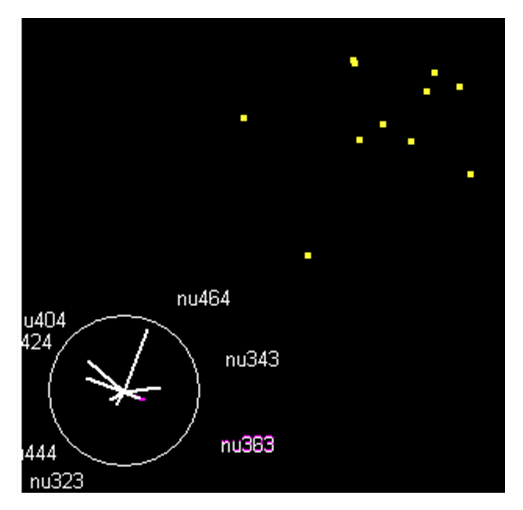
\includegraphics{2DTour_fcc.eps}
%\caption{{G\footnotesize GOBI} snapshot of multidimensional fcc
%RP�s. The axes are not located at the origin of the hypersphere,
%which is approximately in the center of the group of RP's, but are
%always located toward the lower left corner of the plot
%window.}\label{2DTour}
%\end{figure}

%\begin{figure}
%\scalebox{.45}{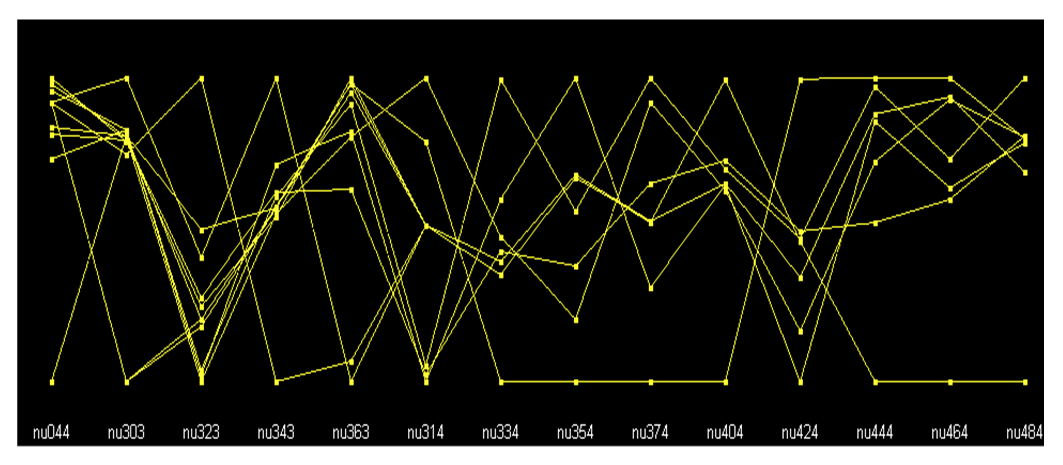
\includegraphics{parallelCoordinate_fcc.eps}}
%\caption{Parallel coordinate plot of fcc RP�s.  Correlations in
%parameters nu044--nu363 show preferred regions of potential
%parameter space.}\label{parallelCoordinate}
%\end{figure}

Interpreting the potential coefficients in Table~\ref{RPTop} is
analogous to describing multipole interactions. These multipoles
include contributions from all interaction modes and are not limited
to electrostatic  interactions. In the case of tetrahedral molecules
the octopole ($\ell_i=3$) is the first nonzero multipole.
Coefficients such as $\nu_{0,3,3}$ and $\nu_{0,4,4}$ where $\ell_i$
or $\ell_j$ is zero represent an octopole or hexadecapole
interacting with the zeroth pole and are the crystal field
coefficients. As the basis functions may also be used as quantum
basis sets, the $\mb{\nu}$ may be calculated \emph{ab initio} and
have been given physical interpretations via symmetry-adpated
perturbation theory~\cite{Avoird94}.  For instance, although
dispersion and induction force can be found in all components of
$\mb{\nu}$, electrostatic forces contribute only to
$\nu^{n_\sigma,n_\mu}_{\ell_i,\ell_i+\ell_j,\ell_j}$~\cite{Stone84}
such as $\nu_{3,6,3}$, $\nu_{3,7,4}$, and $\nu_{4,8,4}$.

One drawback of using the algorithm in
Sec.~\ref{Computational_Strategy} is that, by finding the maximum
energy difference between a phase and all others, the RP's of
neighboring phases tend to be spread apart.  This is because an RP
is a vector representing a region in a space, not a unique set of IP
parameters.  Homologous series of molecules (\emph{i.e.} CF$_4$,
CCl$_4$, CBr$_4$, CI$_4$) are expected to show trends in $\mb{\nu}$
space. If members of homologous series have different crystal
structures, then they have different RP's. However, different RP's
are widely spread by our algorithm. Therefore RP's of homologous
series are often widely spaced, even if the molecules are expected
to have similar intermolecular potentials. This hides the expected
trends among homologues.

Correlations are evident in reference lattice assignments.
%Examples include the
%$\mathrm{CX}_4$ series composed of five homologues,
%$\mathrm{CI}_4$ [CSD structure ZZZKDW01~\cite{Pohl82}],
%$\mathrm{CBr}_4$ [CSD structure CTBROM~\cite{More77}],
%$\mathrm{CCl}_4$ [CSD structure CARBTC~\cite{Piermarini73}],
%$\mathrm{CF}_4$ [CSD structure TFMETH02~\cite{Fitch93}],
%$\mathrm{CD}_4$, in five structures, 121a (ZZZKDW01), 15f,f,f,f
%(CTBROM), 14e (QUGBOJ), 15e (REKYUB), 64d,f (METHANEIII), that all
%pack in one reference lattice, fcc. An organometallic example is
An example of this is a series of molecules with molecular formula
$\mathrm{C}_{16}\mathrm{H}_{36}\mathrm{X}_{4}\mathrm{In}_4\mathrm{N}_4$
where $\mathrm{X}$ is Cl, Br, or I. The first two structures, 14e
MECKUA and 12i MECKOU,
%[CSD structure MECKUA~\cite{Grabowy00} and CSD structure MECKOU~\cite{Grabowy00}]
pack in an fcc reference lattice while
the last, 11e MECKIO, %[CSD structure MECKIO~\cite{Grabowy00}],
packs in a tetragonal reference lattice intermediate between fcc and
bcc which is slightly closer to the bcc reference lattice. This
indicates at least the translational part of homologue potentials is
similar and that small changes in the atomic constituency can
slightly alter the intermolecular potential (IP), but significantly
alter crystal structure. This is consistent with experience that
similar molecules often have very different crystal structures
despite similar intermolecular potentials. GPDs acknowledge this by
placing the seemingly disparate structures close to one another in
IP parameter space.

In \cite{McClurg05} we noted that structures 195a and 197a were very
similar to higher symmetry structures (215a and 217a). If the
molecules remained tetrahedral then the crystal would retain higher
symmetry but the reported atomic coordinates indicate a minor
molecular distortion reducing the space group symmetry. Assuming
that the reported space group is correct, these structures require a
symmetry-breaking pathway from sc and bcc with a minimal truncation
manifold of $\ell_i^{\mathrm{max}}=6$ or 9 (depending on the
potential-dependent transition pathway taken). In contrast to these
high manifold requirements most pathways require a third or fourth
manifold basis set. In view of the success of finding RP's using
only the two first manifolds ($\ell_i^{\mathrm{max}}=3$ or 4) for
all other molecules in the data set, it seems unlikely such a large
number of rapidly oscillating basis functions would be required to
properly describe the intermolecular potential for these structures.
It seems more likely that, barring a Jahn-Teller crystal distortion,
the crystal symmetry may have been underspecified when reported to
the CSD.

\subsection{Extensions and Features of the Methodology}
\label{extensions}

We now discuss some of the ways to improve the model and algorithms.
An issue affecting the numerical accuracy of the RP is how large a
library of alternate crystal structures is needed to localize the RP
in $\mb{\nu}$ space. In our previous work~\cite{Mettes04} we
considered just the high-symmetry point isotropy subgroups and in
this work have followed suit since these are the most
common~\cite{Stokes88}. Recall that space group IR's are indexed by
reciprocal space vectors~\cite{Kovalev93,Zak69}. There are the same
number of $\mb{k}$ points in reciprocal space as there are unit
cells in the crystal and there is a correspondence between $\mb{k}$
points and supercell patterns in the crystal. Experimental
structures are supercells in their reference lattice. As nearly all
experimental structures contain a relatively small number of
clustered parent lattice unit cells as sublattices,
symmetry-breaking occurs at $\mb{k}$ vectors corresponding to this
small cluster.  These are $\mb{k}$ vectors at high symmetry points
in the reference lattice Brillouin zone. If the experimental
structure has a unit cell which is large or flattened/elongated,
however, $\mb{k}$ vectors corresponding to this larger or
longer/flatter group of parent lattice unit cells will be on high
symmetry lines and planes. Symmetry breaking pathways for experimental lattices
pertaining to bcc and fcc reference lattices in the appendix show that some experimental structures contain
large or non-clustered parent lattice unit cells such as 15f,f,f,f
or 152b and their $\mb{k}$ vectors therefore are from high-symmetry
plane and line IR's. Although these cases are less common, such
isotropy subgroups could be included in the candidate lattices in
Sec.~\ref{collection}. Providing such additional structures in the
library would place additional constraints on the RP for the
observed structures and therefore further localize the RP for each
observed structure at the expense of a much larger library.

In Sec.~\ref{collection} we chose to consider only isotropy
subgroups with one occupied Wyckoff point. This is a commonly used
simplification.~\cite{Verwer98} We have also discarded coupled IR
isotropy subgroups for the same reason. Our method could be extended
to include library structures with multiple Wyckoff points and those
from coupled IRs, although the computational demands are much higher
because of the larger set of candidate lattices and so we do not
pursue it here. The effect would be to further localize the RPs of
each phase, again at the expense of a much larger library.

Although tetrahedral molecules are used in the current example to
reverse engineer the IP, any molecular point group could be used
without a dramatic increase in the number of potential coefficients
$\mb{\nu}$ in the first two non-trivial manifolds. This is because
the absence of IP coefficients in lower manifolds for high-symmetry
molecules is offset by the larger number of parameters in higher
manifolds. Consider the number of basis functions in the first two
non-trivial manifolds of $I_h$
(the icosahedral group) %, $T_d$ (the tetrahedral group),
and $C_1$ (the point group of no special symmetry). These are the
highest and lowest molecular point group symmetries, respectively.
The first three manifolds of $I_h$ containing a totally symmetric
molecular representation are the zeroth, sixth, and tenth manifolds.
The number of potential coefficients is seven on the sixth manifold,
$\{\nu_{6,0,6}^{1,1}$, $\nu_{6,2,6}^{1,1}$,
...$\nu_{6,12,6}^{1,1}\}$, eleven on the tenth manifold,
$\{\nu_{10,0,10}^{1,1}$, $\nu_{10,2,10}^{1,1}$,
...$\nu_{10,20,10}^{1,1}\}$, and seven for the cross manifolds,
$\{\nu_{6,4,10}^{1,1}$, $\nu_{6,6,10}^{1,1}$,
...$\nu_{6,16,10}^{1,1}\}$.  There are also two crystal field
coefficients, $\{\nu_{0,6,6}^{1,1}$, $\nu_{0,10,10}^{1,1}\}$, giving
a total of 27 potential coefficients for $I_h$.  For $C_1$ the first
three manifolds are the zeroth, first, and second. The coefficients
on the first manifold are $\{\nu_{1,0,1}^{n_\sigma,n_\mu}$,
$\nu_{1,2,1}^{n_\sigma,n_\mu}\}$. Although there are three copies of
the totally symmetric molecular representation on the first manifold
and therefore the molecular frame indices $\sigma$ and $\mu$ in
Eq.~\ref{re:eq:vij2} go over $\{1,2,3\}$, we are free to choose the
standard orientation for the molecule corresponding to Euler angles
$\{0,0,0\}$.  If it is chosen with the IP major axis parallel to the
laboratory z-axis then only one of these is nonzero. This leaves two
coefficients $\{\nu_{1,0,1}^{1,1}$, $\nu_{1,2,1}^{1,1}\}$. If the
molecular minor axis in the standard orientation is oriented
parallel to the laboratory x-axis only four of the $\sigma$ and
$\mu$ are nonzero in the second manifold. This leaves 48
coefficients on the second manifold,
$\{\nu_{2,0,2}^{n_\sigma,n_\mu}$, $\nu_{2,2,2}^{n_\sigma,n_\mu}$,
$\nu_{2,4,2}^{n_\sigma,n_\mu}\}$. With five additional crystal field
coefficients $\{\nu^{1,1}_{0,1,1}$, $\nu^{1,n_\mu}_{0,2,2}\}$ and
eight cross manifold coefficients $\{\nu^{1,n_\mu}_{1,1,2}$,
$\nu^{1,n_\mu}_{1,3,2}\}$ the total number of coefficients on the
first three manifolds of $C_1$ is 60, an increase of roughly twofold
from highly symmetrical $I_h$. This shows that although this method
has been applied to tetrahedral molecules, it is applicable to other
molecular point group symmetries with only a modest change in the
number parameters.

\begin{table}
\caption{Comparison of the cumulative number of parameters in
potential for a truncation at a given manifold for two truncation
strategies and three molecular point groups.}\label{tab:truncation}
\begin{tabular}{ccccccccc}
\multicolumn{4}{c}{Direct Truncation} & &\multicolumn{4}{c}{$\ell$ sum Truncation}\\
\cline{1-4}\cline{6-9}\\
$\ell_i$ & $C_1$ & $T_d$ & $I_h$ & & $\ell_i+\ell_j$ & $C_1$ &
$T_d$ & $I_h$\\
\cline{1-4}\cline{6-9}\\
0  & $^*$  & $^*$  & $^*$  & & 0  & $^*$  & $^*$ & $^*$ \\
1  & 3  & 0  & 0  & & 1  & 1  & 0 & 0 \\
2  & 60 & 0  & 0  & & 2  & 6  & 0 & 0 \\
3  &    & 5  & 0  & & 3  & 15 & 1 & 0 \\
4  &    & 10 & 0  & & 4  &    & 1 & 0 \\
6  &    &    & 8  & & 6  &    & 6 & 1 \\
10 &    &    & 19 & & 10 &    &   & 8 \\
\cline{1-4}\cline{6-9}\\
\end{tabular}
\\$^*$ There is one isotropic basis function for $\ell_i=\ell_j=0$ in
each case, but it does not drive orientational ordering.
\end{table}

Throughout we have implemented a simple direct cutoff truncation
scheme in which a doubly infinite summation is cut off at a maximum
manifold number $\ell_i^\mathrm{max}$.  An alternative is the
manifold-sum cutoff in which we truncate such that $\ell_i+\ell_j\le
\ell^\mathrm{max}$. This truncation would include smoother functions
before more rapidly oscillating ones which is consistent with our
expectations of lower-energy electronic contributions to the
potential. Also the number of potential parameters increases at a
slower rate with this truncation. This is shown in
Table~\ref{tab:truncation} for both truncation schemes where we
compare the cumulative number of parameters for the $C_1$, $T_d$,
and $I_h$ point groups at different manifolds. The truncation method
used in this study is a square truncation of the double sum while
the alternative is a triangular truncation. The manifold sum
truncation adds new parameters into the potential more slowly than
single manifold truncation. Therefore, the 15 coefficients used here
are sufficient but may not be necessary. Further investigation of
global phase diagrams with $\ell$-sum truncation is needed to test
this hypothesis. This is important since lower dimensional GPDs
would be easier to construct and to use.

From the foregoing discussion we have seen 15 coefficients are
sufficient to reverse engineer our dataset of experimental
structures.  We have not investigated if a linear combination would
be better.  Principle component analysis could be used to identify
linear combinations of basis functions that better fit molecules. It
is possible that less than 15 coefficients are necessary.

%Although Table~\ref{RPTop} shows that a potential can be
%successfully reverse engineered which produces the experimentally
%observed structure with remarkably few terms,

%As noted in Sec.~\ref{truncation}, some of the molecules in
%Table~\ref{group_theory} break symmetry due to coupled IR's.
%Although examples of coupled IR's exist in nature, they are less
%common than single IR's~\cite{Hatch87}. From experience gained in
%creating GPD's, coupled order parameters typically exist in a
%region of parameter space \emph{one dimension lower} than the
%surrounding phases. An example in 3D is that the coupled IR phase
%is the \emph{line} separating single IR \emph{surfaces} on the
%unit sphere. GPD calculations show phases with coupled IR's
%possess \emph{significantly} lower free energies than adjacent
%neighbors. An important consequence in crystal structure
%prediction is an interaction potential sufficient to produce one
%of these structures requires a very precise $\mb{\nu}$ vector.
%This may be an important contributor to the lack of success of
%crystal structure prediction codes~\cite{Motherwell02}. It also
%underscores the utility of GPD's in accurately assessing
%intermolecular forces.

\subsection{Conclusions}

We have shown that a molecular crystal global phase diagram (GPD)
with a small number of reference lattices derived
in~\cite{McClurg05} can summarize the experimental data using a
modest number of IP parameters. The data set is diverse enough to
test the GPD's ability to classify a wide range of space groups
using a common intermolecular potential. Just as the van Konynenburg
global phase diagram classification based on the simple van der
Waals equation of state is nonetheless widely used to classify the
phase behavior of real binary mixtures, molecular crystal global
phase diagrams may be useful in elucidating phase behavior of a
variety of real substances and, in turn, used to develop novel
intermolecular potentials and materials.

%\begin{acknowledgments}
%This work received financial support from the American Chemical
%Society - Petroleum Research Fund (PRF \#41774-AC10).
%%
%Computational resources maintained by the University of Minnesota
%Supercomputer Institute were used for portions of this research.
%\end{acknowledgments}

\ack{This work received financial support from the American Chemical Society - Petroleum Research Fund (PRF \#41774-AC10).
%
Computational resources maintained by the University of Minnesota Supercomputer Institute were used for portions of this research.}

\appendix
Appendix matter has been placed in the supplementary material.

%\begin{references}
%\reference{Author, A. \& Author, B. (1984). \emph{Journal} \textbf{Vol},
%first page--last page.}
%\end{references}
%\bibliographystyle{normalTitle}
%\bibliographystyle{plain}
%\bibliography{thesisbib}
\referencelist

     %-------------------------------------------------------------------------
     % TABLES AND FIGURES SHOULD BE INSERTED AFTER THE MAIN BODY OF THE TEXT
     %-------------------------------------------------------------------------

These tables list group theoretical symmetry-breaking pathways for experimental
lattices belonging to the bcc, hcp, sc, and A5$^\prime$ reference lattices.

\begin{table}
\caption{Group theoretical symmetry-breaking pathways of experimental lattices from the
bcc reference lattice. Classified by space group IR and order
parameter direction, each pathway shows the point group IR and
minimal manifold of SO(3) in Eq.~(\ref{re:eq:vij2}) required to
achieve it.  The order parameter directions are given in an abbreviated form in the
notation of Stokes and
Hatch~\cite{Stokes02a}.}\label{pathwaysBCC} \footnotesize
\begin{tabular}{lllll}\hline
Pathway & S.~G.~IR & OP Dir. & P.~G.~IR & $\ell^{\mathrm{req'd}}$  \\
\hline
229a $\rightarrow$ 217a & $\Gamma_2^-$ & P1 & $A_{2u}$ & 3 \\

229a $\rightarrow$ 161a & $H_5^- \oplus \Gamma_2^-$ & P3 $\oplus$ P1 & $T_{2u} \oplus
A_{2u}$ & 3 \\
& $H_5^- \oplus \Gamma_4^-$ & P3 $\oplus$ P3 & $T_{2u} \oplus
T_{1u}$ &3 \\
& $H_5^- \oplus H_4^+$ & P3 $\oplus$ P3 & $T_{2u} \oplus T_{1g}$
& 4 \\
& $H_4^+ \oplus \Gamma_2^-$ & P3 $\oplus$ P1 & $T_{1g} \oplus A_{2u}$ & 4 \\
& $H_4^+ \oplus \Gamma_4^-$ & P3 $\oplus$ P3 & $T_{1g} \oplus T_{1u}$ & 4\\
& $H_5^- \oplus H_2^+$ & P3 $\oplus$ P1 & $T_{2u} \oplus A_{2g}$
& 6\\
& $H_2^+ \oplus \Gamma_4^-$ & P1 $\oplus$ P3 & $A_{2g} \oplus T_{1u}$ & 6 \\
& $H_1^- \oplus \Gamma_4^-$ & P1 $\oplus$ P3 & $A_{1u} \oplus
T_{1u}$ & 9 \\
& $H_1^- \oplus H_4^+$ & P1 $\oplus$ P3 & $A_{1u} \oplus T_{1g}$
& 9\\

229a $\rightarrow$ 62c (RIMMOP) & $N_2^- \oplus N_4^+$ & P1
$\oplus$ P1 & $A_{2u},E_u,T_{1u} \oplus T_{1g},T_{2g}$ & 4 \\

229a $\rightarrow$ 60c,d (YIMWEW) & $^*$\\

229a $\rightarrow$ 11e & $N_4^- \oplus N_2^-$ & P1 $\oplus$ P1 & $T_{1u},T_{2u} \oplus
A_{2u},E_u,T_{1u}$ & 3\\
&  & P1 $\oplus$ C1  \\
& $N_2^- \oplus \Gamma_4^+$ & P1
$\oplus$ P2 & $A_{2u},E_u,T_{1u} \oplus T_{1g}$ & 4\\
&  & C1 $\oplus$ P2 \\
& $N_2^- \oplus \Gamma_5^+$ & P1 $\oplus$ C2 & $A_{2u},E_u,T_{1u}
\oplus T_{2g}$ & 4 \\
& & C1 $\oplus$ C2 \\
& $N_4^- \oplus \Gamma_4^+$ & P1 $\oplus$ P2 & $T_{1u},T_{2u}
\oplus T_{1g}$ & 4 \\
& $N_4^- \oplus \Gamma_5^+$ & P1 $\oplus$ C2 & $T_{1u},T_{2u}
\oplus T_{2g}$ & 4 \\

229a $\rightarrow$ 2i (MEZDIE01) & $N_1^-\oplus\Gamma_4^+$ &
P1 $\oplus$ S1 & $A_{1u},E_u,T_{2u} \oplus T_{1g}$ & 4\\
& $N_1^-\oplus\Gamma_5^+$ & P1 $\oplus$ S1 & $A_{1u},E_u,T_{2u}
\oplus T_{2g}$ & 4\\
& $N_2^-\oplus\Gamma_4^+$ & P1 $\oplus$ S1 & $A_{2u},E_u,T_{1u}
\oplus T_{1g}$ & 4 \\
& $N_2^-\oplus\Gamma_5^+$ & P1 $\oplus$ S1 & $A_{2u},E_u,T_{1u}
\oplus T_{2g}$ & 4 \\
& $N_3^-\oplus\Gamma_4^+$ & P1 $\oplus$ S1 & $T_{1u},T_{2u} \oplus
T_{1g}$ & 4\\
& $N_3^-\oplus\Gamma_5^+$ & P1 $\oplus$ S1 & $T_{1u},T_{2u} \oplus
T_{2g}$ & 4\\
& $N_4^-\oplus\Gamma_4^+$ & P1 $\oplus$ S1 & $T_{1u},T_{2u} \oplus
T_{1g}$ & 4\\
& $N_4^-\oplus\Gamma_5^+$ & P1 $\oplus$ S1 & $T_{1u},T_{2u} \oplus
T_{2g}$ & 4\\

229a $\rightarrow$ 2iii & $H_4^-$ & S1 & $T_{1u}$ & 3\\
& H5- & S1 & $T_{2u}$ & 3\\
\hline
\end{tabular}
\end{table}

\begin{table}
\caption{Group theoretical symmetry-breaking pathways of
experimental lattices for the hcp reference
lattice.}\label{pathwaysHCP}%\tiny
\begin{tabular}{lllll}\hline
Pathway & S.~G.~IR & OP Dir. & P.~G.~IR & $\ell^{\mathrm{req'd}}$ \\
\hline
194c $\rightarrow$ 176h & $K_4$ & P1 & $E^\prime$ & 3 \\
194c $\rightarrow$ 165d & $A_2$ & P3 & $A_2^\prime,A_1^\prime$ & 3 \\
194c $\rightarrow$ 147d & $\Gamma_3^+ \oplus \Gamma_2^+$ & P1$ \oplus$ P1 & $A_2^{\prime\prime}\oplus A_2^\prime$ & 3 \\
& $\Gamma_4^+ \oplus \Gamma_2^+$ & P1$ \oplus$ P1 & $A_1^{\prime\prime}\oplus A_2^\prime$ & 4 \\
& $\Gamma_4^+ \oplus \Gamma_3^+$ & P1$ \oplus$ P1 & $A_1^{\prime\prime}\oplus A_2^{\prime\prime}$ & 4 \\
194c  $\rightarrow$ 14e DOCNIS & $M_1^-\oplus \Gamma_2^+$ & P1$ \oplus$ P1 & $A_1^{\prime\prime},E^{\prime\prime} \oplus A_2^\prime $ & 3 \\
& $M_1^- \oplus \Gamma_2^+$ & C1$ \oplus$ P1 & $A_1^{\prime\prime},E^{\prime\prime} \oplus A_2^\prime$ & 3 \\
& $M_1^- \oplus \Gamma_5^+$ & P1$ \oplus$ C1 & $A_1^{\prime\prime},E^{\prime\prime} \oplus E^{\prime}$ & 3 \\
& $M_1^- \oplus \Gamma_5^+$ & C1$ \oplus$ C1 & $A_1^{\prime\prime},E^{\prime\prime} \oplus E^\prime$ & 3 \\
& $M_2^- \oplus \Gamma_2^+$ & P1$ \oplus$ P1 & $A_2^{\prime\prime},E^{\prime\prime} \oplus A_2^\prime$ & 3 \\
& $M_2^- \oplus \Gamma_2^+$ & C1$ \oplus$ P1 & $A_2^{\prime\prime},E^{\prime\prime} \oplus A_2^\prime$ & 3 \\
& $M_2^- \oplus \Gamma_5^+$ & P1$ \oplus$ C1 & $A_2^{\prime\prime},E^{\prime\prime} \oplus E^\prime$ & 3 \\
& $M_2^- \oplus \Gamma_5^+$ & C1$ \oplus$ C1 & $A_2^{\prime\prime},E^{\prime\prime} \oplus E^\prime$ & 3 \\
& $M_2^- \oplus M_1^- $ & P1$ \oplus$ P1 & $A_2^{\prime\prime},E^{\prime\prime} \oplus A_1^{\prime\prime},E^{\prime\prime}$ & 3 \\
& $M_2^- \oplus M_1^-$ & C1$ \oplus$ C1 & $A_2^{\prime\prime},E^{\prime\prime} \oplus A_1^{\prime\prime},E^{\prime\prime}$ & 3 \\
194c  $\rightarrow$ 14e CARBTC & $M_2^+ \oplus \Gamma_6^+$ & P1$ \oplus$ P1 &  $A_2^\prime,E^\prime \oplus E^{\prime\prime}$ & 3 \\
& $M_2^+ \oplus \Gamma_6^+$ & P1$ \oplus$ P1  &  $A_2^\prime,E^\prime \oplus E^{\prime\prime}$ & 3 \\
& $M_2^+ \oplus \Gamma_3^+$ & P1$ \oplus$ P1 &  $A_2^\prime,E^\prime \oplus A_2^{\prime\prime}$ & 4 \\
& $M_4^+ \oplus \Gamma_3^+$ & P1$ \oplus$ P1 &   $A_1^{\prime\prime},E^{\prime\prime} \oplus A_2^{\prime\prime}$ & 4 \\
& $M_4^+ \oplus \Gamma_5^+$ & P1$ \oplus$ C1 &  $A_1^{\prime\prime},E^{\prime\prime} \oplus E^\prime$ & 4 \\
& $M_4^+ \oplus \Gamma_6^+$ & P1$ \oplus$ P1 &  $A_1^{\prime\prime},E^{\prime\prime} \oplus E^{\prime\prime}$ & 4 \\
& $M_4^+ \oplus M_2^+$  & P1$ \oplus$ P1 & $A_1^{\prime\prime},E^{\prime\prime} \oplus A_2^\prime,E^\prime$ & 4 \\
\hline
\end{tabular}
\end{table}

\begin{table}
\caption{Group theoretical symmetry-breaking pathways of
experimental lattices for the sc reference
lattice.}\label{pathwaysSC}%\tiny
\begin{tabular}{lllll}\hline
Pathway & S.~G.~IR & OP Dir. & P.~G.~IR & $\ell^{\mathrm{req'd}}$  \\
\hline
221a $\rightarrow$ 215a & $\Gamma_2^-$ & P1 & $A_{2u}$ & 3 \\
221a $\rightarrow$ 120c & $R_5^-\oplus \Gamma_2^-$ & P1$ \oplus$ P1 & $T_{2u} \oplus A_{2u}$  & 3 \\
& $R_4^+\oplus \Gamma_2^-$ & P1$ \oplus$ P1 & $T_{1g} \oplus A_{2u}$ & 4 \\
& $R_5^-\oplus R_4^+$ & P1$ \oplus$ P1 & $T_{2u} \oplus T_{1g}$  & 4 \\
& $R_4^+\oplus \Gamma_3^-$ & P1$ \oplus$ P1 & $T_{1g} \oplus E_u$  & 7 \\
& $R_5^-\oplus \Gamma_3^-$ & P1$ \oplus$ P1 & $T_{2u} \oplus E_u$  & 7 \\
\hline
\end{tabular}
\end{table}

\begin{table}
{Group theoretical symmetry-breaking pathways of experimental lattices
for the A5$^\prime$ reference lattice.} \label{pathwaysA5}
\begin{tabular}{lllll}\hline
Pathway & S.~G.~IR & OP Dir. & P.~G.~IR & $\ell^{\mathrm{req'd}}$  \\
\hline
141a $\rightarrow$ 141a & $\Gamma_1^+$ &  P1 & $A_{1}$ & 3 \\
141a $\rightarrow$ 15e & $\Gamma_5^+$ &  P3 & $E$ & 3 \\
141a $\rightarrow$ 14e & $\Gamma_3^+ \oplus M_3 $ &  P1 $\oplus$ P3 & $A_{2} \oplus E $ & 3 \\
& $\Gamma_3^+ \oplus M_4 $ &  P1 $\oplus$ P3 & $A_{2} \oplus E$ &  3\\
& $M_3 \oplus M_4 $ &  P3 $\oplus$ P3 & $E \oplus E$ &  3\\
&  $\Gamma_4^+ \oplus M_3 $ &  P1 $\oplus$ P3 & $B_{1} \oplus E$ &  4\\
& $\Gamma_4^+ \oplus M_4 $ &  P1 $\oplus$ P3 & $B_{1} \oplus E$ &  4\\
\hline
\end{tabular}
\end{table}

\end{document}                    % DO NOT DELETE THIS LINE
%%%%%%%%%%%%%%%%%%%%%%%%%%%%%%%%%%%%%%%%%%%%%%%%%%%%%%%%%%%%%%%%%%%%%%%%%%%%%%
